In this tutorial, we introduce QMCPy \cite{QMCPy2020a}  by an example. QMCPy can be installed with \texttt{pip install qmcpy} or cloned from the  \href{https://github.com/QMCSoftware/QMCSoftware}{QMCSoftware GitHub repository}.

Consider the problem of integrating the Keister function \cite{Kei96} with respect to a $d$-dimensional Gaussian measure: 
\begin{align*}
    f(\vx) &= \pi^{d/2} \cos(||\vx||), \qquad \vx \in \reals^d, \qquad \vX \sim \mathcal{N}(\vzero_d,\mI_d/2),  
\\ \mu  &=  \Ex[f(\vX)] := \int_{\reals^d} f(\vx) \, \pi^{-d/2} \exp( - ||\vx||^2) \,  \dif \vx 
\\     &= \bigintss_{[0,1]^d} \pi^{d/2}  \cos\left(\sqrt{ \frac 12 \sum_{j=1}^d\Phi^{-1}(x_j)}\right)  \, \dif \vx. 
\end{align*}
where $||\vx||$ is the \href{https://en.wikipedia.org/wiki/Norm_(mathematics)}{Euclidean norm}, $\mI_d$ is the $d$-dimensional identity matrix, and 
$\Phi$ denotes the standard normal cumulative distribution function. When $d=2$, $\mu \approx 1.80819$ and we can visualize the Keister function and realizations of the sampling points depending on the tolerance values, $\varepsilon$, in the following figure.

\begin{center}
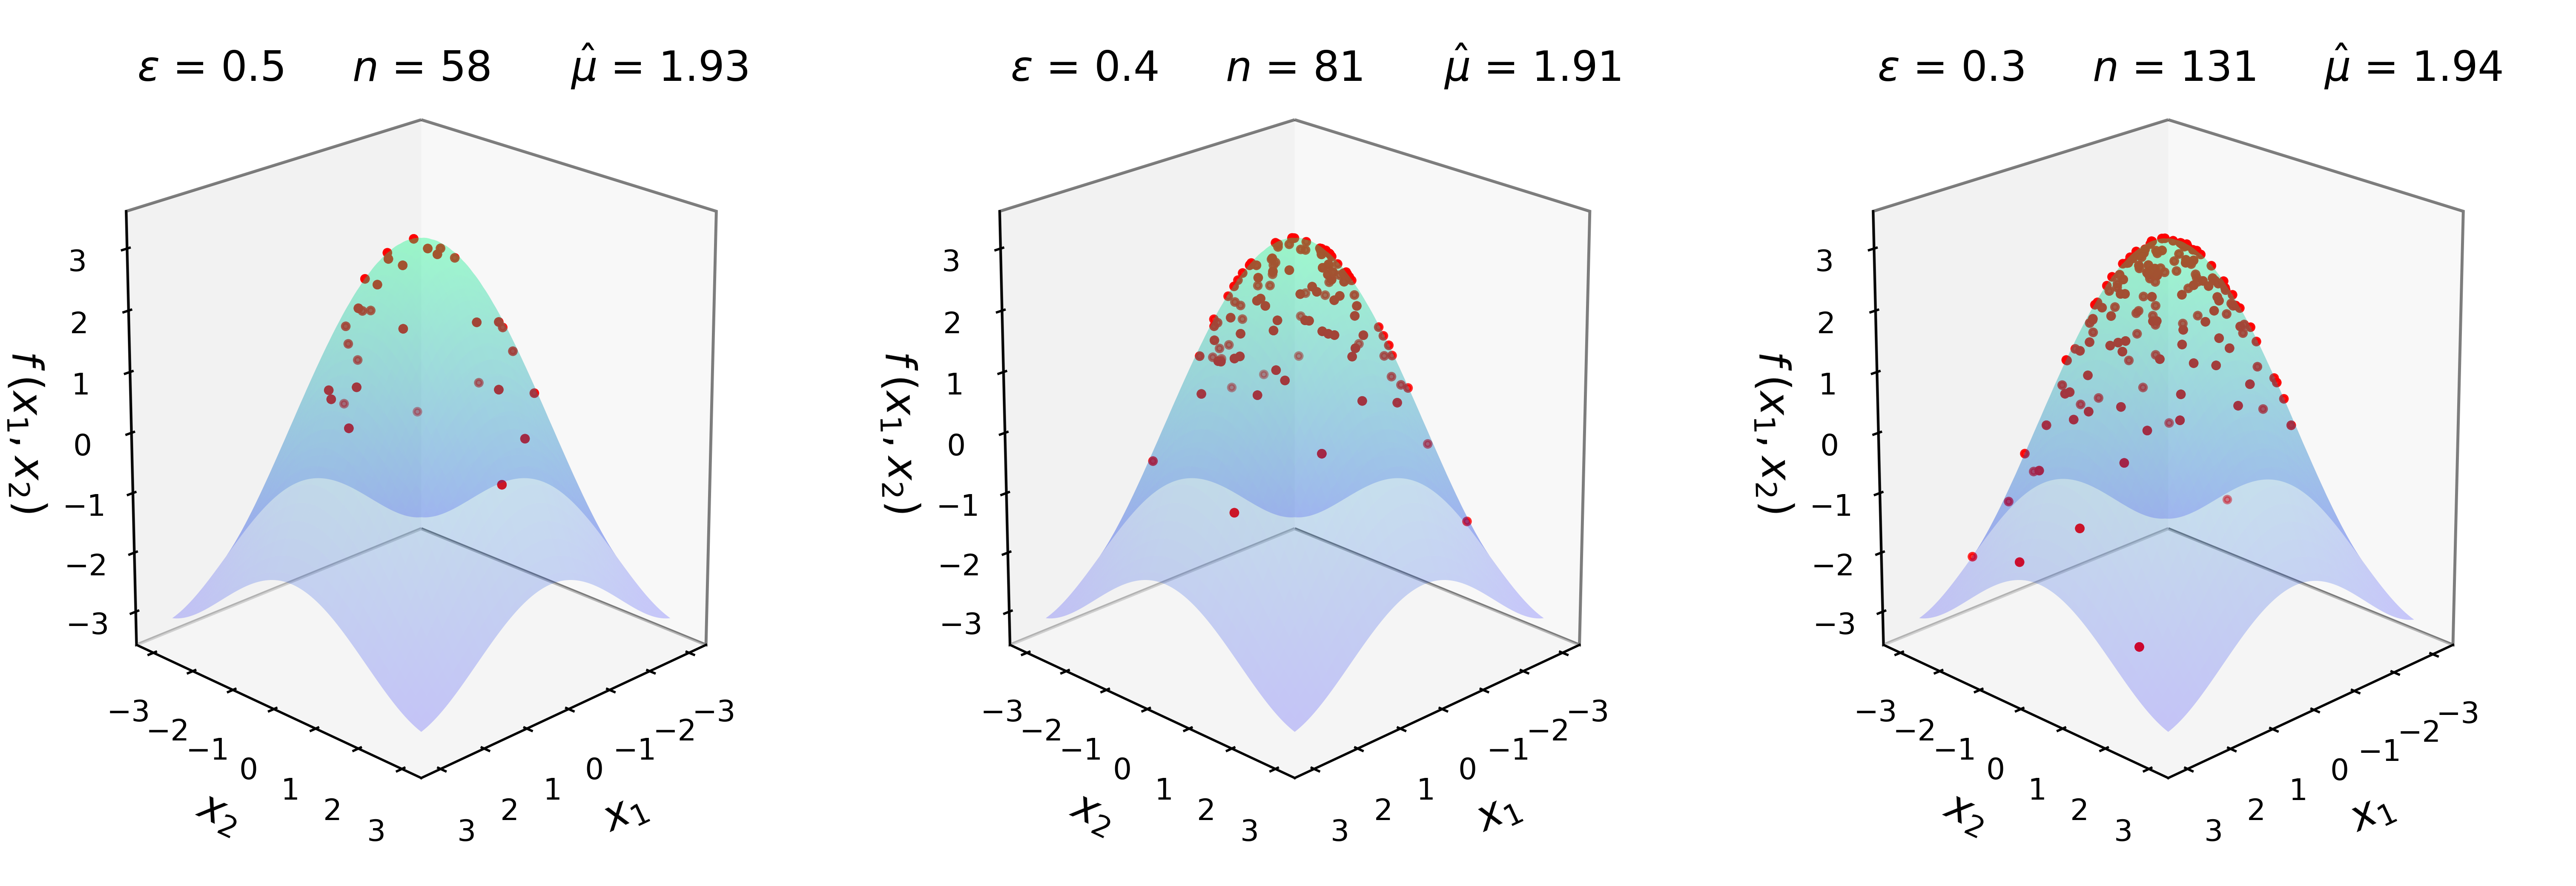
\includegraphics[width=1\textwidth]{Quickstart/Three_3d_SurfaceScatters.png}      
\end{center}   

The Keister function is implemented below with help from NumPy~\cite{numpy} in the following code snippet:
\lstinputlisting[style=Python]{Quickstart/snip1.py}

In addition to our Keister integrand and Gaussian true measure, we must select a discrete distribution, and a stopping criterion~\cite{HicEtal18a}. The stopping criterion determines the number of points at which to evaluate the integrand in order for the mean approximation to be accurate within a user-specified error tolerance, $\varepsilon$. The discrete distribution determines the sites at which the integrand is evaluated.

For this Keister example, we select the lattice sequence as the discrete distribution and corresponding cubature-based stopping criterion~\cite{JimHic16a}. The discrete distribution, true measure, integrand, and stopping criterion are then constructed within the QMCPy framework below. 

\lstinputlisting[style=Python]{Quickstart/snip2.py}

Calling \texttt{integrate} on the \texttt{stopping\_criterion} instance returns the numerical solution and a data object. Printing the data object will provide a neat summary of the integration problem. For details of the output fields, refer to the online, searchable QMCPy Documentation at \href{https://qmcpy.readthedocs.io/en/latest/algorithms.html#module-qmcpy.integrand.keister}{https://qmcpy.readthedocs.io/}
\lstinputlisting[style=Python]{Quickstart/snip3.py}

This guide is not meant to be exhaustive but rather a quick introduction to the QMCPy framework and syntax. In an upcoming blog, we will take a closer look at low-discrepancy sequences such as the lattice sequence from the above example.  
